% Chapter 4

\chapter{Ensayos y resultados} % Main chapter title

\label{Chapter4} % For referencing the chapter elsewhere, use \ref{Chapter4} 
\label{resultados}

%----------------------------------------------------------------------------------------

\section{Montaje}

En esta sección se describe y expone el diseño físico final del dispositivo, comenzando exclusivamente por los circuitos de alimentación y posteriormente con el armado final.

\subsection{Conexiones y PCB}

El esquema de conexiones final para el circuito de alimentación del capturador de imágenes es el siguiente:

\begin{figure}[htbp]
    \centering
    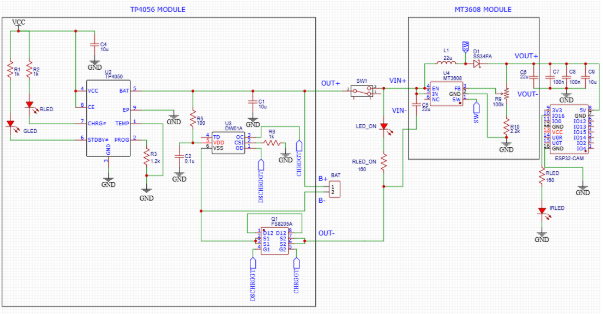
\includegraphics[width=0.9\textwidth]{figuras/esquemacapturador.png}
    \caption{Esquema de conexiones para la PCB del circuito capturador}
    \label{esquemacapturador}
\end{figure}

Incluye los módulos \emph{TP4056}, \emph{MT3608}, un switch intermedio entre ellos para desconectar manualmente el dispositivo, y finalmente el zócalo donde se inserta la \emph{ESP32}, al cual se le conecta el LED IR para normalizar la iluminación en el ojo.

Al tener los módulos comerciales, el esquemático final de la PCB se reduce a este simple esquema:

\begin{figure}[htbp]
    \centering
    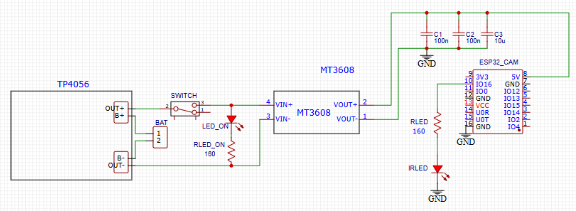
\includegraphics[width=0.9\textwidth]{figuras/esquemacapturadorsimple.png}
    \caption{Esquema simplificado de la PCB del circuito capturador}
    \label{esquemacapturadorsimple}
\end{figure}

La entrada del \emph{TP4056} se conecta mediante USB-C, por lo que no se incluye en el esquemático de la PCB.

A su vez, el esquema de conexiones de la placa que actuará como servidor web es el siguiente:

\begin{figure}[htbp]
    \centering
    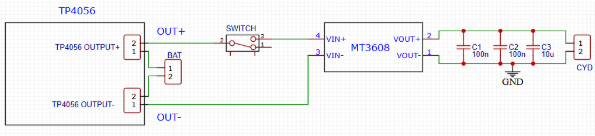
\includegraphics[width=0.9\textwidth]{figuras/esquemareceptor.png}
    \caption{Esquema simplificado de la PCB del circuito servidor}
    \label{esquemareceptor}
\end{figure}

Prácticamente igual al anterior, sin los diodos LED ni la \emph{ESP32-CAM}. En su lugar se coloca una bornera doble de la que saldrán cables para alimentar a la CYD.

\keyword{Diseño de PCB}

A continuación se muestran imágenes del diseño de las PCBs para ambos dispositivos, diseñados en el software web \emph{EasyEDA}.

\begin{figure}[htbp]
    \centering
    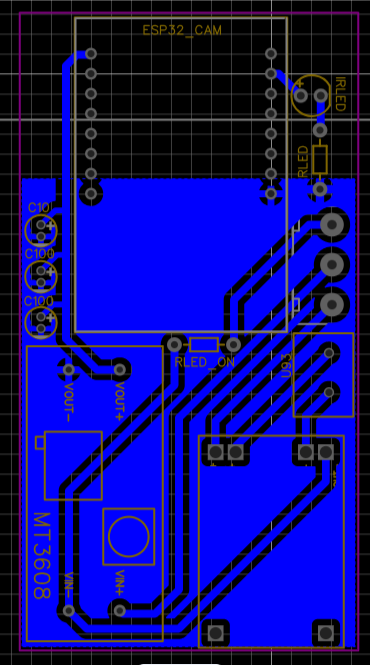
\includegraphics[width=0.4\textwidth]{figuras/layoutcapturador.png}
    \caption{Layout de la PCB del circuito capturador}
    \label{layoutcapturador}
\end{figure}

En lugar de colocar directamente el LED de encendido en la PCB, se opta por utilizar una bornera de 3 terminales para conectarlo externamente. Esto para poder decidir con más libertad su posición exacta en el dispositivo final.

\begin{figure}[htbp]
    \centering
    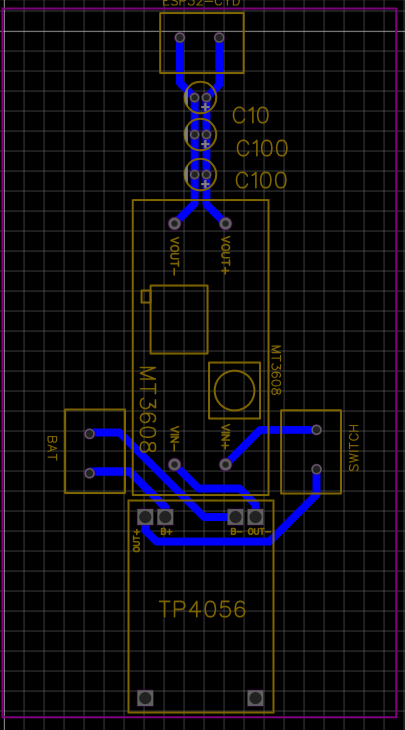
\includegraphics[width=0.4\textwidth]{figuras/layoutservidor.png}
    \caption{Layout de la PCB del circuito servidor}
    \label{layoutservidor}
\end{figure}

\subsection{Ensamblaje del prototipo}

\section{Pruebas de Software}

\subsection{Pruebas del tracker} 

\subsection{Pruebas unitarias}

\section{Pruebas de Hardware}

(Cambiar todas las imagenes por tablas)

\section{Pruebas de rendimiento}

\section{Pruebas de integración}